% \documentclass[12pt]{article}
\usepackage[left=0.25cm,top=1cm,right=0.25cm,bottom=1cm]{geometry}
\textwidth = 20cm
\hoffset = -1cm
\usepackage[utf8]{inputenc}
\usepackage[spanish,es-tabla]{babel}
\usepackage[autostyle,spanish=mexican]{csquotes}
\usepackage[tbtags]{amsmath}
\usepackage{nccmath}
\usepackage{amsthm}
\usepackage{amssymb}
\usepackage{graphicx}
\usepackage{standalone}
\usepackage[outdir=./]{epstopdf}
\usepackage{siunitx}
\usepackage{physics}
\usepackage{color}
\usepackage{float}
\usepackage{multicol}
%\usepackage{milista}
\usepackage{enumitem}
\usepackage{anyfontsize}
\usepackage{anysize}
\usepackage{enumitem}
\usepackage{capt-of}
\usepackage{bm}
\usepackage{relsize}
\usepackage{placeins}
\usepackage{empheq}
\usepackage{cancel}
\usepackage{wrapfig}
\spanishdecimal{.}
\renewcommand{\baselinestretch}{1.5} 
\renewcommand\labelenumii{\theenumi.{\arabic{enumii}}}
\newcommand{\ptilde}[1]{\ensuremath{{#1}^{\prime}}}
\newcommand{\stilde}[1]{\ensuremath{{#1}^{\prime \prime}}}
\newcommand{\ttilde}[1]{\ensuremath{{#1}^{\prime \prime \prime}}}
\newcommand{\ntilde}[2]{\ensuremath{{#1}^{(#2)}}}


% \geometry{top=1.25cm, bottom=1.5cm, left=1.25cm, right=0.8cm}
% %\usepackage{showframe}

\documentclass[12pt]{article}
\usepackage[utf8]{inputenc}
\usepackage[T1]{fontenc}
\usepackage[spanish,es-lcroman]{babel}
\usepackage{amsmath}
\usepackage{amsthm}
\usepackage{amsfonts}
\usepackage{amssymb}
\usepackage{physics}
\AtBeginDocument{\RenewCommandCopy\qty\SI}
\usepackage{tikz}
\usepackage{float}
\usepackage{calc}
\usepackage[autostyle,spanish=mexican]{csquotes}
\usepackage[per-mode=symbol]{siunitx}
\usepackage{textcomp, gensymb}
\usepackage{multicol}
\usepackage{enumitem}
\usepackage{hyperref}
\usepackage{setspace}
\usepackage[left=2.00cm, right=2.00cm, top=2.00cm, 
     bottom=2.00cm]{geometry}
% \usepackage{Estilos/ColoresLatex}
\usepackage{makecell}
\usepackage{subcaption}
\usepackage[skip=10pt, indent=30pt]{parskip}
% \usepackage{scalerel}
\usepackage{scalerel}[2016-12-29]
\usepackage{biblatex}
\usepackage{cancel}

\definecolor{ao}{rgb}{0.0, 0.0, 1.0}
\definecolor{burgundy}{rgb}{0.5, 0.0, 0.13}

\hypersetup{
    colorlinks=true,
    linkcolor=ao,
    filecolor=magenta,      
    urlcolor=ao,
}

\newcommand{\ptilde}[1]{\ensuremath{{#1}^{\prime}}}
\newcommand{\stilde}[1]{\ensuremath{{#1}^{\prime \prime}}}
\newcommand{\ttilde}[1]{\ensuremath{{#1}^{\prime \prime \prime}}}
\newcommand{\ntilde}[2]{\ensuremath{{#1}^{(#2)}}}
\newcommand{\pderivada}[1]{\ensuremath{{#1}^{\prime}}}
\newcommand{\sderivada}[1]{\ensuremath{{#1}^{\prime \prime}}}
\newcommand{\tderivada}[1]{\ensuremath{{#1}^{\prime \prime \prime}}}
\newcommand{\nderivada}[2]{\ensuremath{{#1}^{(#2)}}}

\def\stretchint#1{\vcenter{\hbox{\stretchto[440]{\displaystyle\int}{#1}}}}
\def\scaleint#1{\vcenter{\hbox{\scaleto[3ex]{\displaystyle\int}{#1}}}}
\def\scaleiint#1{\vcenter{\hbox{\scaleto[6ex]{\displaystyle\iint}{#1}}}}
\def\scaleiiint#1{\vcenter{\hbox{\scaleto[6ex]{\displaystyle\iiint}{#1}}}}
\def\scaleoint#1{\vcenter{\hbox{\scaleto[3ex]{\displaystyle\oint}{#1}}}}
\def\bs{\mkern-12mu}

\newcommand{\textocolor}[2]{\textbf{\textcolor{#1}{#2}}}
\sisetup{per-mode=symbol}
\decimalpoint
\sisetup{bracket-numbers = false}
\newlength{\depthofsumsign}
\setlength{\depthofsumsign}{\depthof{$\sum$}}
\newcommand{\nsum}[1][1.4]{% only for \displaystyle
    \mathop{%
        \raisebox
            {-#1\depthofsumsign+1\depthofsumsign}
            {\scalebox
                {#1}
                {$\displaystyle\sum$}%
            }
    }
}

\AtBeginDocument{\RenewCommandCopy\qty\SI}
\ExplSyntaxOn
\msg_redirect_name:nnn { siunitx } { physics-pkg } { none }
\ExplSyntaxOff

\numberwithin{equation}{section}

\linespread{1.15}

\renewcommand{\labelenumii}{\theenumii}
\renewcommand{\theenumii}{\theenumi.\arabic{enumii}.}

\emergencystretch=1em

\title{Examen Extraordinario \\ \large {Matemáticas Avanzadas de la Física}  \vspace{-3ex}}
% \author{M. en C. Gustavo Contreras Mayén}
\date{ }

\begin{document}
\vspace{-4cm}
\maketitle
\fontsize{14}{14}\selectfont

\begin{enumerate}
%Referencia Hassani
\item Una esfera conductora de calor de radio $a$ está compuesta por dos hemisferios con un espacio infinitesimal aislante entre ellos, como se muestra en la figura (\ref{fig:figura2}). Las mitades superior e inferior de la esfera están en contacto con baños térmicos de temperaturas $+ T_{1}$ y $-T_{1}$, respectivamente. La esfera de radio $a$ está dentro de otra esfera conductora de calor de radio $b$ con una temperatura $T_{2}$. Encuentra la temperatura en los puntos:
\begin{enumerate}[label=\alph*)]
\item Dentro de la esfera interior,
\item En la región entre las dos esferas y
\item Por fuera de la esfera exterior.
\end{enumerate} 
\begin{figure}[H]
    \centering
    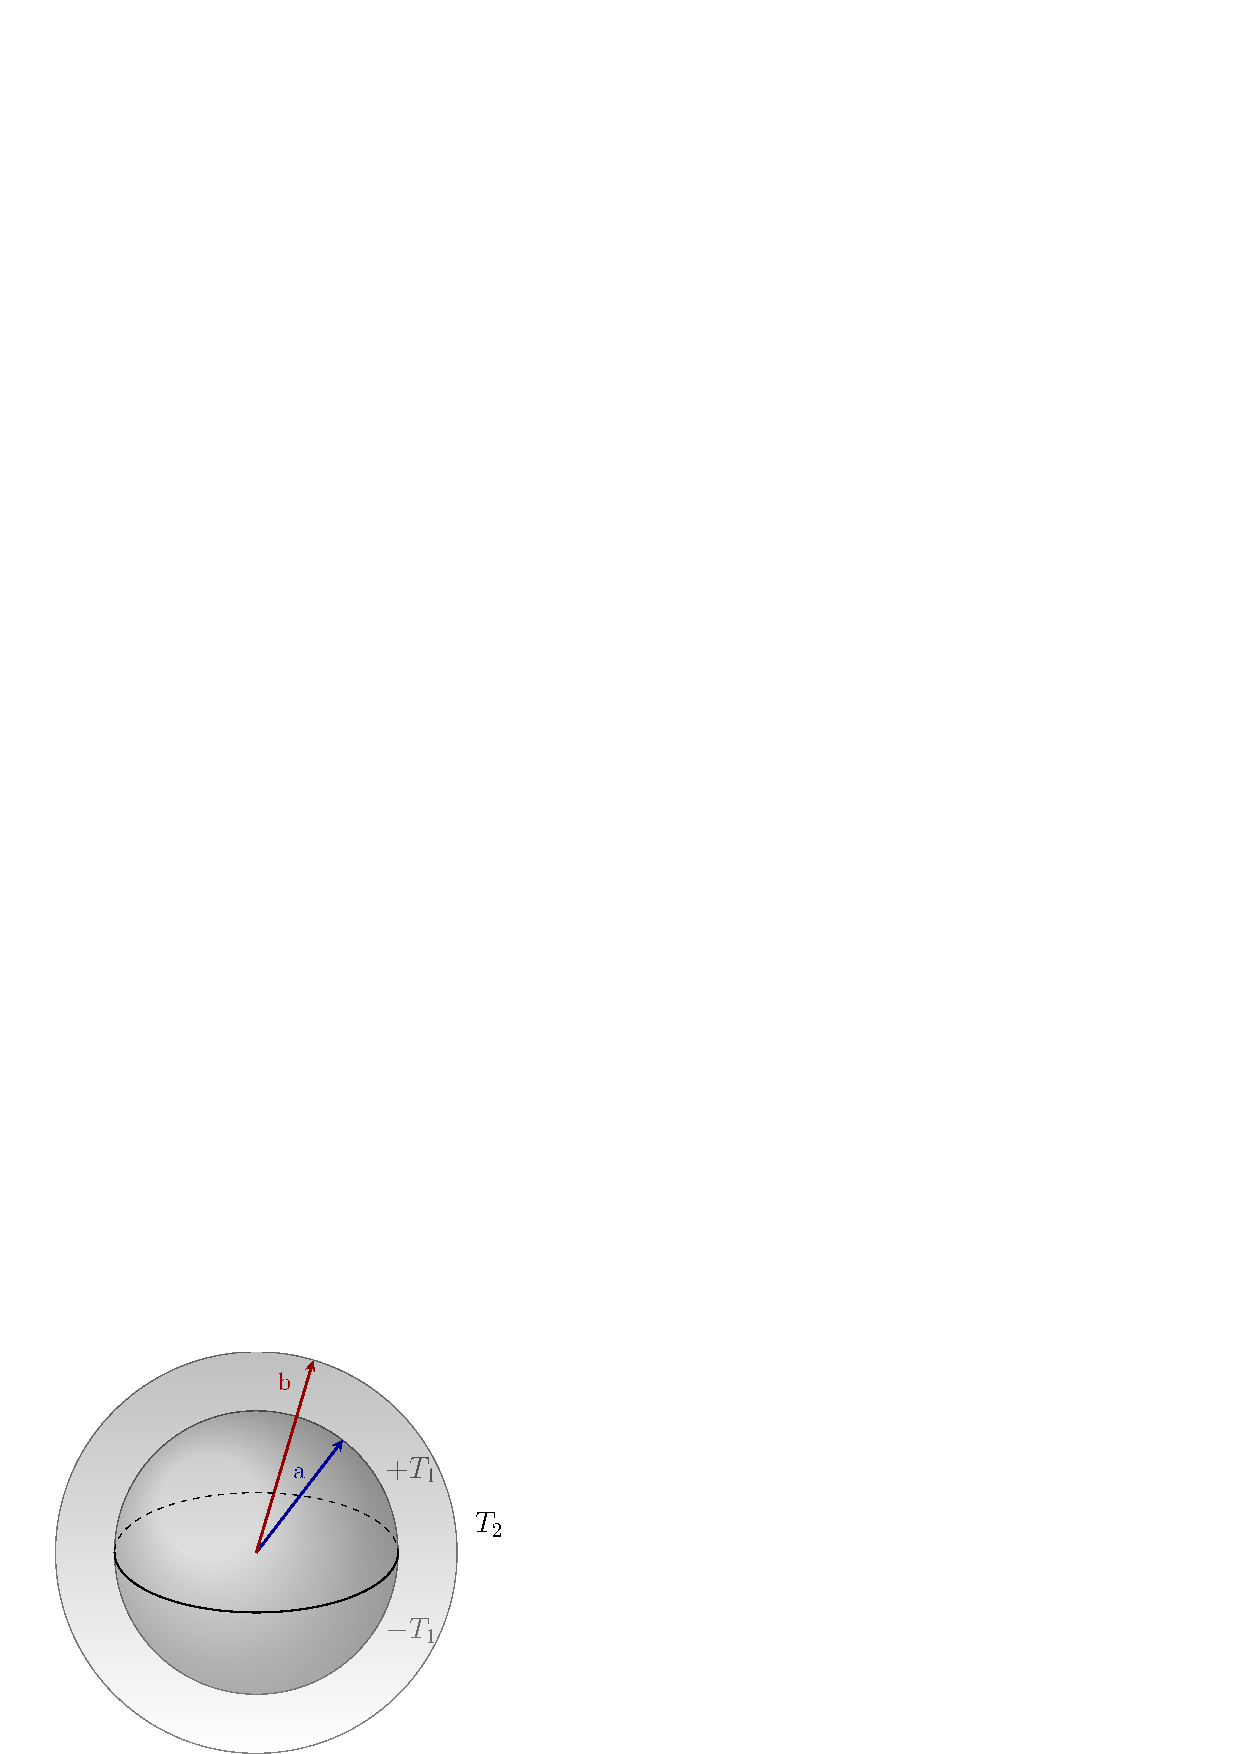
\includegraphics[scale=0.7]{Figuras/esfera1.pdf}
    %\includestandalone{esfera1}
    \caption{Los hemisferios de la esfera interior se encuentran a diferentes temperatura.}
    \label{fig:figura2}
\end{figure}
%Referencia. Arfken. Cap. 12 Legendre functions. Problem 12.3.11
\item La amplitud de una onda dispersada está dada por
\begin{align*}
f (\theta) = \dfrac{1}{k} \sum_{\ell = 0}^{\infty} (2 \, \ell + 1) \, \exp(i \, \delta_{\ell}) \, \sin \delta_{\ell} \, P_{\ell} (\cos \theta)
\end{align*}
Donde $\theta$ es el ángulo de dispersión, $\ell$ es el valor propio del momento angular, $\hbar \, k$ es el momento incidente, y $\delta_{\ell}$ es el desplazamiento de fase producido por el potencial central que está haciendo la dispersión. La sección transversal total es 
\begin{align*}
\sigma_{\text{tot}} = \scaleint{6ex} \abs{f(\theta)}^{2} \dd{\Omega}
\end{align*}
Demuestra que:
\begin{align*}
\sigma_{\text{tot}} = \dfrac{4 \, \pi}{k^{2}} \nsum_{\ell=0}^{\infty} (2 \, \ell + 1) \, \sin^{2} \delta_{\ell}
\end{align*}
%Referencia Cap. 12 Legendre functions. Problem 12.5.2
\item Demuestra que
\begin{align*}
P_{2n}^{1} (0) &= 0 \\
P_{2n+1}^{1} (0) &= (-1)^{n} \, \dfrac{(2n + 1)!}{(2^{2} \, n!)^{2}} = (-1)^{2} \, \dfrac{(2n + 1)!!}{(2n)!!}
\end{align*}
Utilizando cada uno de los siguientes métodos:
\begin{enumerate}[label=\alph*)]
\item Usando la relación de recurrencia.
\item Expandiendo la función generatriz.
\item Con la fórmula de Rodrigues.
\end{enumerate}
\item La transición de probabilidad entre dos estados $\psi_{m}$ y $\psi_{n}$ del oscilador armónico cuántico, depende de que el valor de la siguiente integral sea:
\begin{align*}
\scaleint{6ex}_{-\infty}^{\infty} x \; e^{-x^{2}} \; H_{n} (x) \, H_{m}(x) \dd{x} = \sqrt{\pi} \; 2^{n-1} \; n! \; \delta_{m,n-1} + \sqrt{\pi} \; 2^{n} \; (n+1)! \; \delta_{m,n+1}
\end{align*}
Obtén explícitamente este valor. El resultado demuestra que cada transición puede ocurrir solamente entre estados con niveles de energía adyacentes, \break \hfill $m = n \pm 1$.
%Referencia. Arfken. Cap. 12 Legendre functions. Problem 12.6.3
\item En la teoría de Coulomb para la excitación del núcleo aparece el armónico esférico $Y_{l}^{m} \left( \dfrac{\pi}{2}, 0 \right)$. Demuestra que
\begin{align*}
Y_{l}^{m} \left( \dfrac{\pi}{2}, 0 \right) = \begin{cases}
= \left( \dfrac{2 \, l +1}{4 \, \pi} \right)^{1/2} \, \dfrac{\left[ (l - m)! \, (l + m)! \right]^{1/2}}{(l - m)!! \, (l + m)!!} \, (-1)^{(l + m)/2} & \mbox{ para } l + m \mbox{ par} \\[0.5em]
= 0 & \mbox{para } l + m \mbox{ impar}
\end{cases}
\end{align*}
%Referencia Jackson 4.1
\item Considera una distribución de carga como se muestra en la figura (\ref{fig:figura_multipolo_01}):
\begin{figure}[H]
    \centering
    \includegraphics[scale=0.7]{Figuras/multipolo_01.pdf}
    \caption{Distribución de cargas para el ejercicio.}
    \label{fig:figura_multipolo_01}
\end{figure}
\item Demuestra que la densidad de carga en coordenadas esféricas está dada por la expresión:
\begin{align*}
\rho = \dfrac{q}{2 \, \pi \, a^{2}} \, \delta(r -a) [\delta (\cos \theta - 1) + \delta (\cos \theta + 1)] - \dfrac{2 \, q}{4 \, \pi \, r^{2}} \delta(r)
\end{align*}
%Ref. Patra (2018) Ejercicios Cap. (1) (1)
\item Calcula la transformada de Fourier de la siguiente función:
\begin{align*}
f (x) = \dfrac{\sin a x}{x}, \hspace{1cm} a > 0
\end{align*}
\end{enumerate}

\end{document}